\section{Field count and PADAR scope}\label{sec:field-count-padar-scope}

\subsection{Field count on a fixed boundary/window}\label{subsec:field-count-fixed-scope}
\paragraph{Scope.}
Fix
\[
\mathcal B=(\partial F,\omega).
\]
All quantities in this subsection are evaluated with respect to \(\mathcal B\).

\paragraph{Variables.}
Let
\[
\mathcal F_{\mathcal B}=\{F_1,\ldots,F_{n_F}\}
\]
be the retained field family, and define
\[
n_F(\mathcal B):=|\mathcal F_{\mathcal B}|.
\]
Here \(n_F\) is the retained field count on the fixed scope \(\mathcal B\). The symbol \(T\) is reserved for duration, account length, or tick count when used. The symbol \(m\) is reserved for cageon order in \(\mathsf C_{2m}\). The symbol \(p\) is reserved for rotor or cycle completion period when used.

\paragraph{Returned-current channels.}
For \(F_i,F_j\in\mathcal F_{\mathcal B}\), write
\[
\ADAR_{i\leftarrow j}
\]
for the returned-current channel from \(F_j\) into \(F_i\). The terms \(\ADAR_{i\leftarrow i}\) are self-return terms. The terms \(\ADAR_{i\leftarrow j}\), \(i\neq j\), are cross-return terms.

\paragraph{Poly term.}
The poly term entering the PADAR calculation is
\[
K_{\partial F}(\mathcal B)=n_F(\mathcal B)\log n_F(\mathcal B),
\]
with the logarithm base fixed by the declared calculation.

\paragraph{Unit anchor.}
The monon case \(n_F(\mathcal B)=1\) is the unit retained-field anchor:
\[
C_{\mathrm{mono}}:=1.
\]
Coupled-field counting begins at \(n_F(\mathcal B)=2\). Thus
\[
C_{\mathrm{mono}}=1,
\qquad
K_{\partial F}(\mathcal B)=n_F(\mathcal B)\log n_F(\mathcal B)
\quad (n_F\ge2).
\]
Poly is the field-family size in the fixed-scope PADAR calculation.

\begin{figure}[H]
\centering
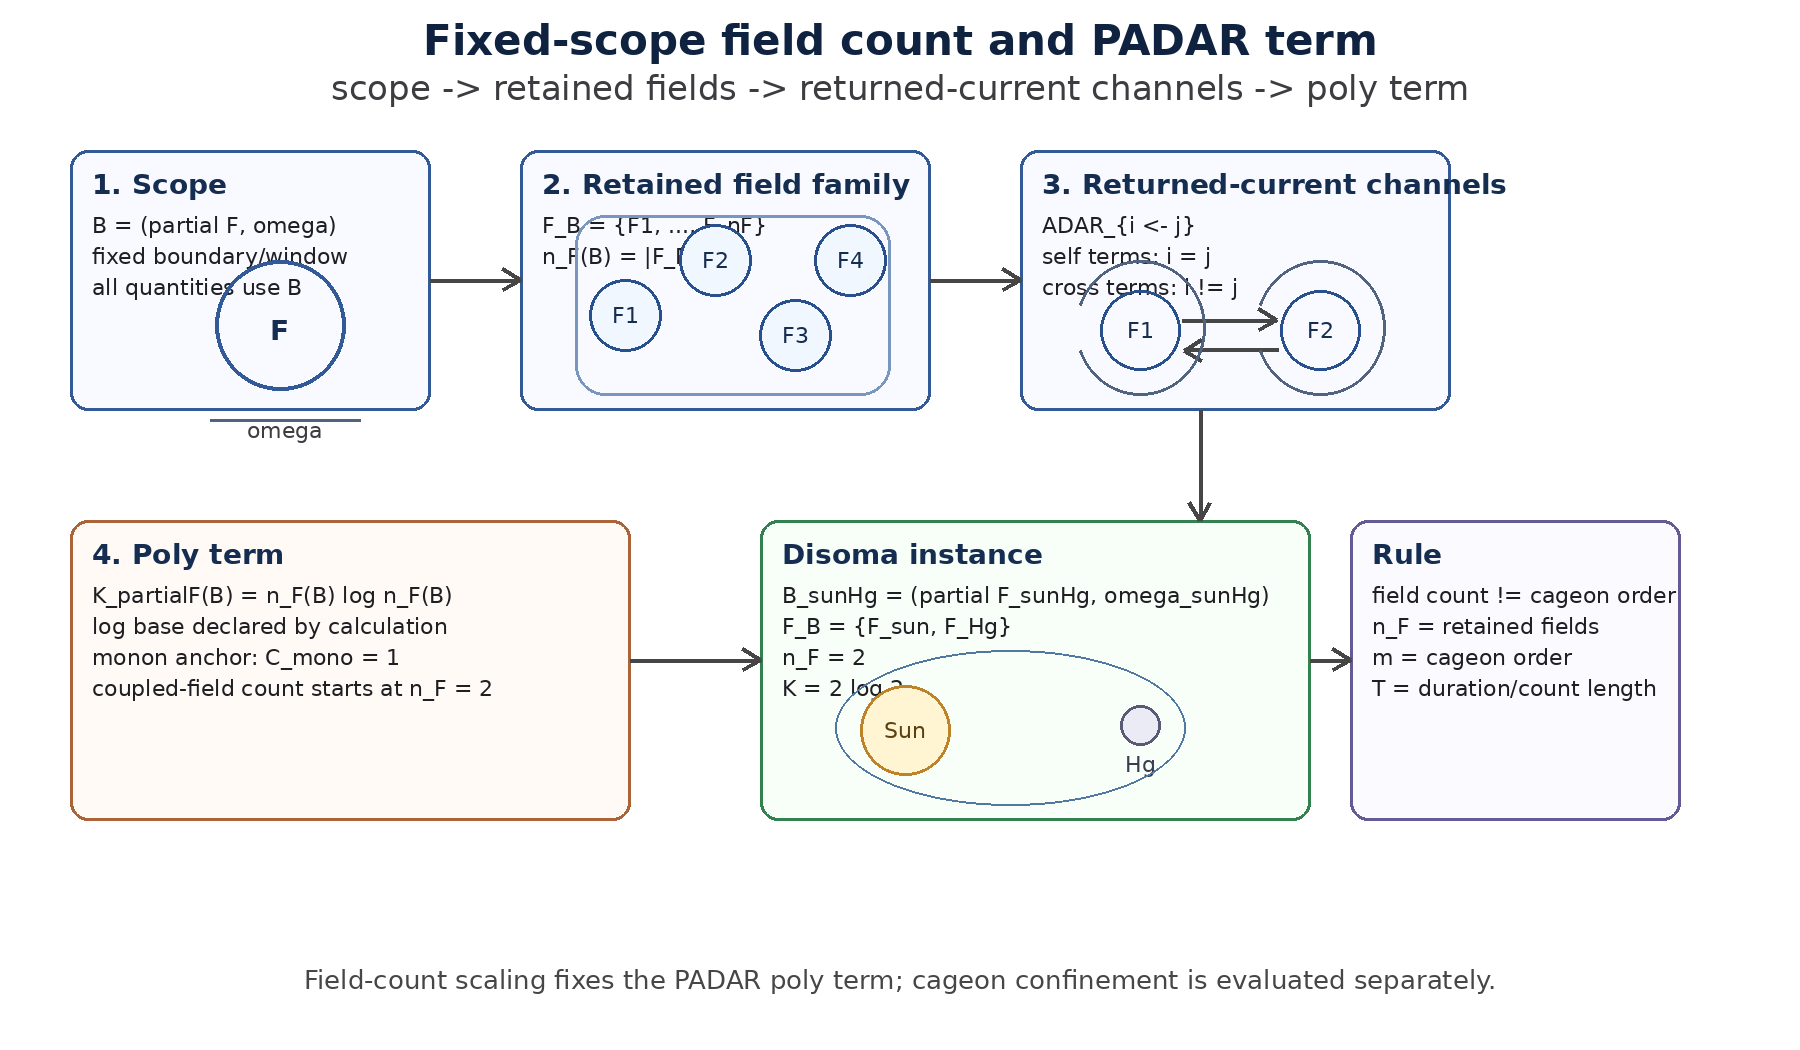
\includegraphics[width=0.98\linewidth]{figures_jpg/v39_21_fixed_scope_field_count.png}
\caption{Field count on a fixed boundary/window. The scope \(\mathcal B=(\partial F,\omega)\) fixes the retained field family \(\mathcal F_{\mathcal B}\), the field count \(n_F\), returned-current channels \(\ADAR_{i\leftarrow j}\), and the PADAR poly term \(K_{\partial F}=n_F\log n_F\).}
\label{fig:v39-fixed-scope-field-count}
\end{figure}

\subsection{Disoma instance}\label{subsec:disoma-instance}
For the Sun--Mercury orbital calculation, fix
\[
\mathcal B_{\odot\mathrm{Hg}}=(\partial F_{\odot\mathrm{Hg}},\omega_{\odot\mathrm{Hg}})
\]
and
\[
\mathcal F_{\mathcal B_{\odot\mathrm{Hg}}}=\{F_\odot,F_{\mathrm{Hg}}\}.
\]
Thus
\[
n_F(\mathcal B_{\odot\mathrm{Hg}})=2,
\]
and
\[
K_{\partial F}(\mathcal B_{\odot\mathrm{Hg}})=2\log 2.
\]
If the calculation declares base \(2\), then
\[
K_{\partial F}^{(2)}(\mathcal B_{\odot\mathrm{Hg}})=2\log_2 2=2.
\]
If the calculation declares trit base, then
\[
K_{\partial F}^{(3)}(\mathcal B_{\odot\mathrm{Hg}})=2\log_3 2.
\]
One retained field is the monon unit anchor. Two retained fields give the disoma field-boundary calculation. \(n_F\) retained fields give the general field-boundary calculation.

\subsection{AFC scale-reuse consequence}\label{subsec:field-count-afc-consequence}
The field-count term
\[
K_{\partial F}(\mathcal B)=n_F(\mathcal B)\log n_F(\mathcal B)
\]
is the field-boundary specialization of the AFC scale-reuse path-counting discipline. It supplies the finite field-family argument of the fixed-scope PADAR calculation.

When the AFC path-complexity bound is cited,
\[
N_T\le \prod_{t=1}^{T}m_t\le c^T T!,
\qquad
\log_3 N_T=O(T\log T),
\]
\(T\) is path or account length scaling. The field-count term \(K_{\partial F}\) uses \(n_F\), the retained field-count size. The two quantities remain distinct.

\subsection{Calculation split}\label{subsec:field-count-cageon-split}
Field-count scaling and cageon confinement are connected by the declared boundary/window, but they are separate calculations. The field-count calculation fixes
\[
\mathcal B\to \mathcal F_{\mathcal B}\to n_F(\mathcal B)\to \ADAR_{i\leftarrow j}\to K_{\partial F}(\mathcal B)\to \PADAR.
\]
Cageon confinement fixes
\[
\mathcal C_{2m}\to P_{\mathcal C}^{\PADAR}\to C_{\mathcal C}^{\mathrm{close}}\to X_{\mathcal C}\to
\text{reclosure / exoshedding / endoshedding / transmutation routing}.
\]
